\section{\simulator: Instantiating \benchmark with Realistic Simulation}
\label{sec:simulation}

\begin{figure}[t]
\captionsetup[subfloat]{labelformat=empty}
\captionsetup[subfloat]{justification=centering}
\centering
\subfloat[][\textbf{\simulator\\ $\mathbf{3.20\pm1.23}$}]{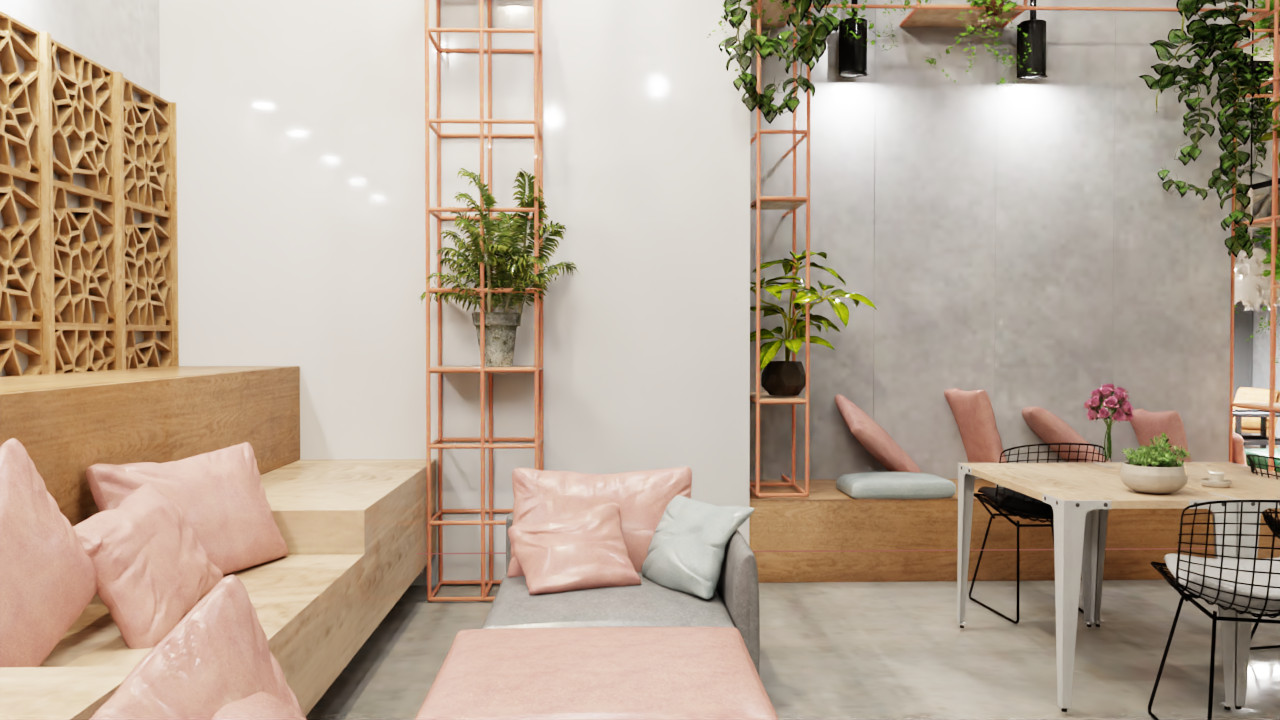
\includegraphics[width=.199\textwidth]{figures/omnigibson/og_sample.jpg}}
\hfill
\subfloat[][Habitat 2.0\\ $1.74\pm1.33$]{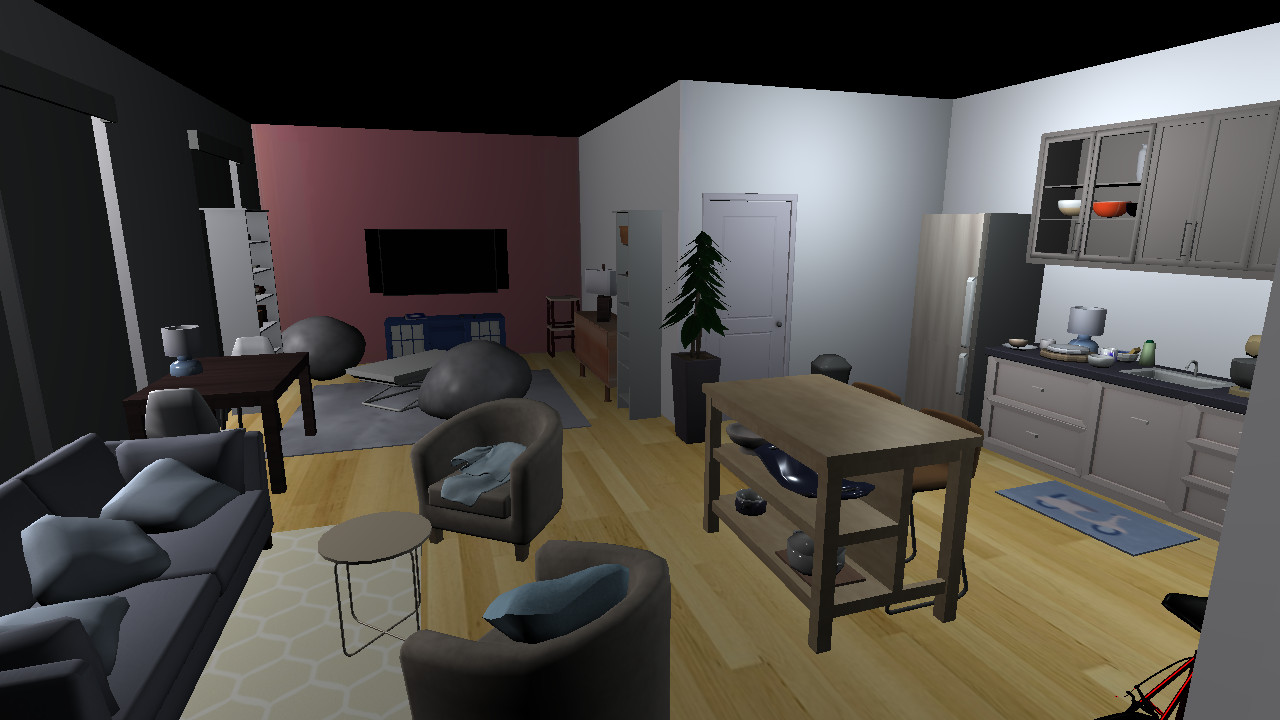
\includegraphics[width=.199\textwidth]{figures/omnigibson/habitat_sample.jpg}}
\hfill
\subfloat[][AI2-THOR\\ $1.73\pm1.37$]{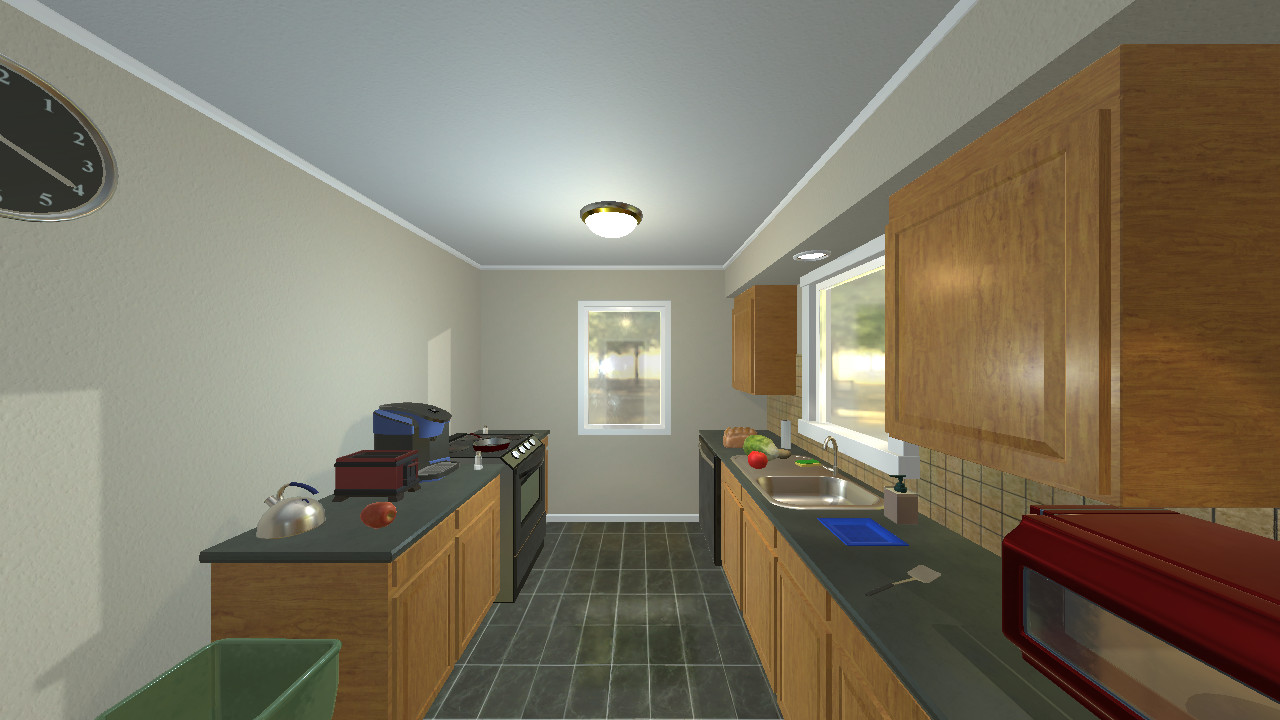
\includegraphics[width=.199\textwidth]{figures/omnigibson/ai2_sample.jpg}}
\hfill
\subfloat[][iGibson 2.0\\ $1.69\pm1.24$]{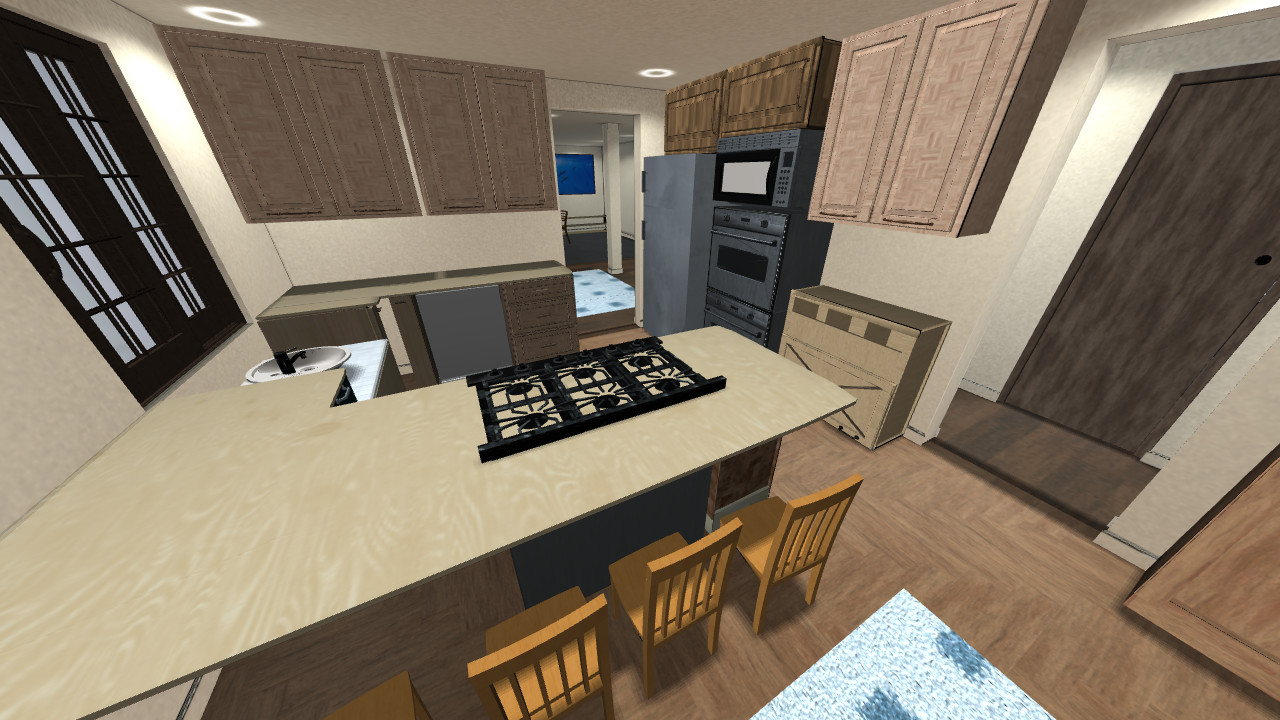
\includegraphics[width=.199\textwidth]{figures/omnigibson/ig2_sample.jpg}}
\hfill
\subfloat[][ThreeDWorld\\ $1.65\pm1.23$]{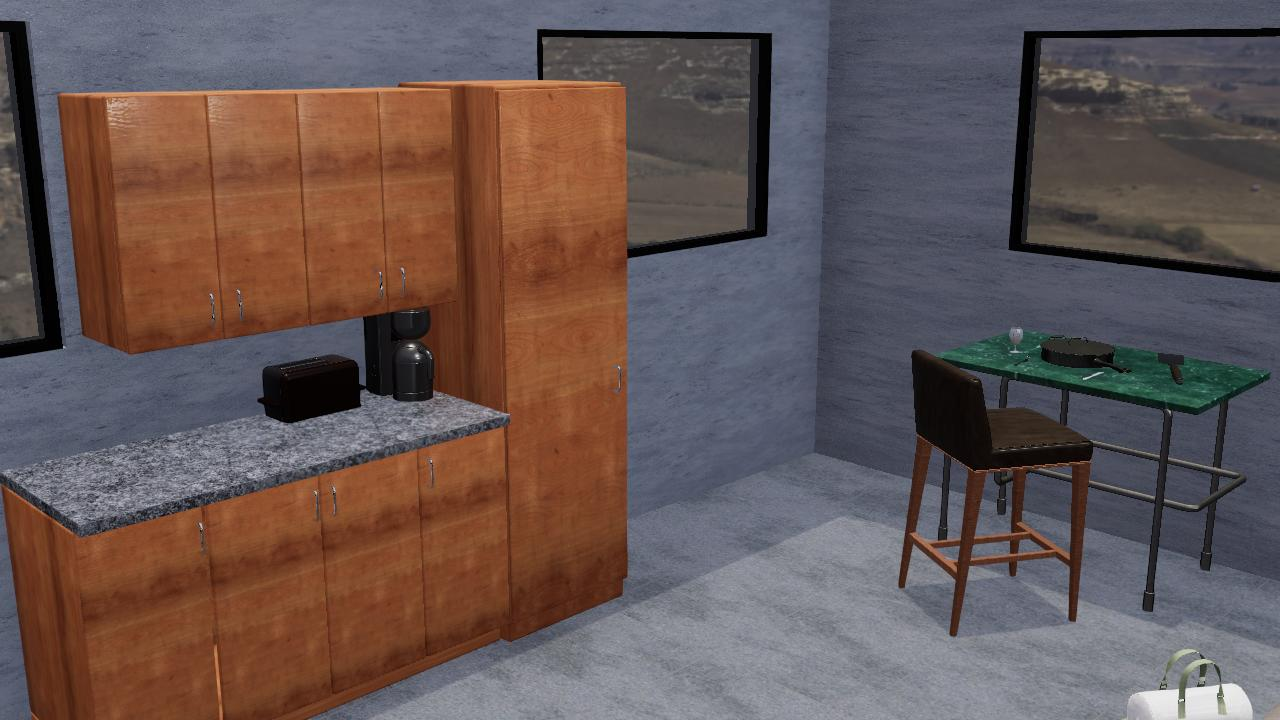
\includegraphics[width=.199\textwidth]{figures/omnigibson/tdw_sample.jpg}}
% \begin{subfigure}{.19\textwidth}
% 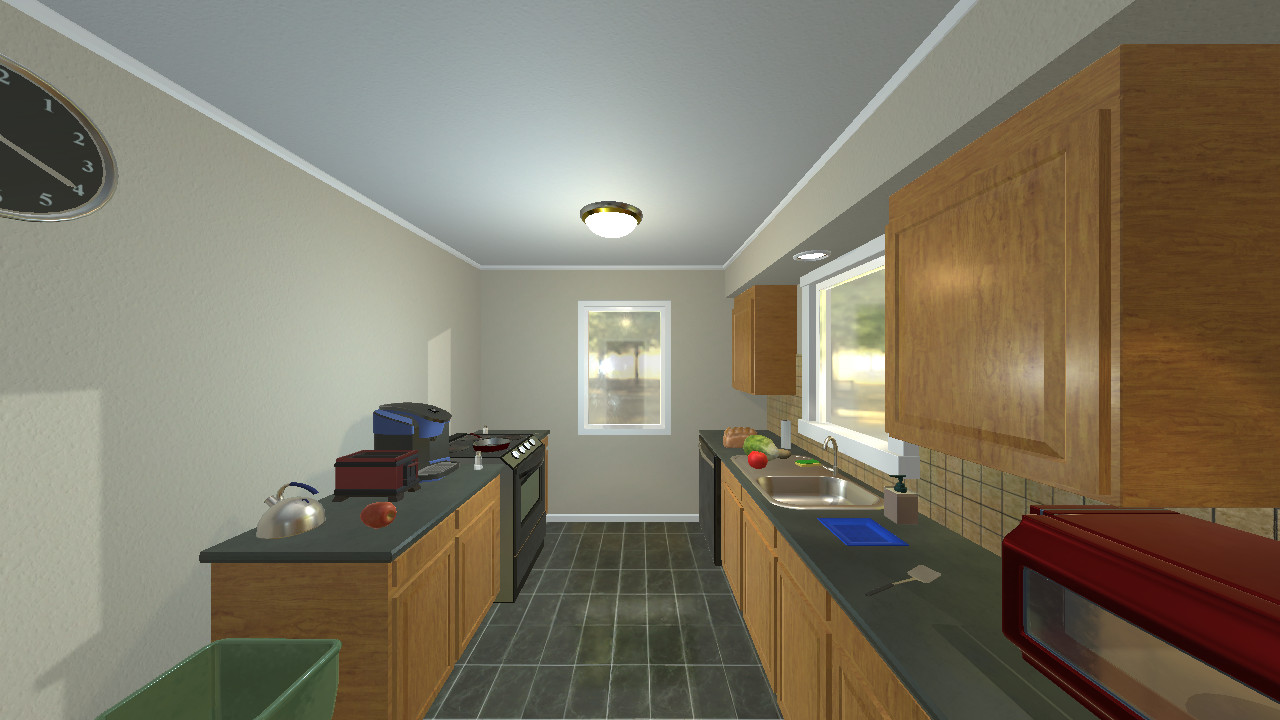
\includegraphics[width=\textwidth]{figures/omnigibson/ai2_sample.png}
% \caption{AI2Thor: $3.27\pm1.25$}
% \end{subfigure}
% \begin{subfigure}{.19\textwidth}
% 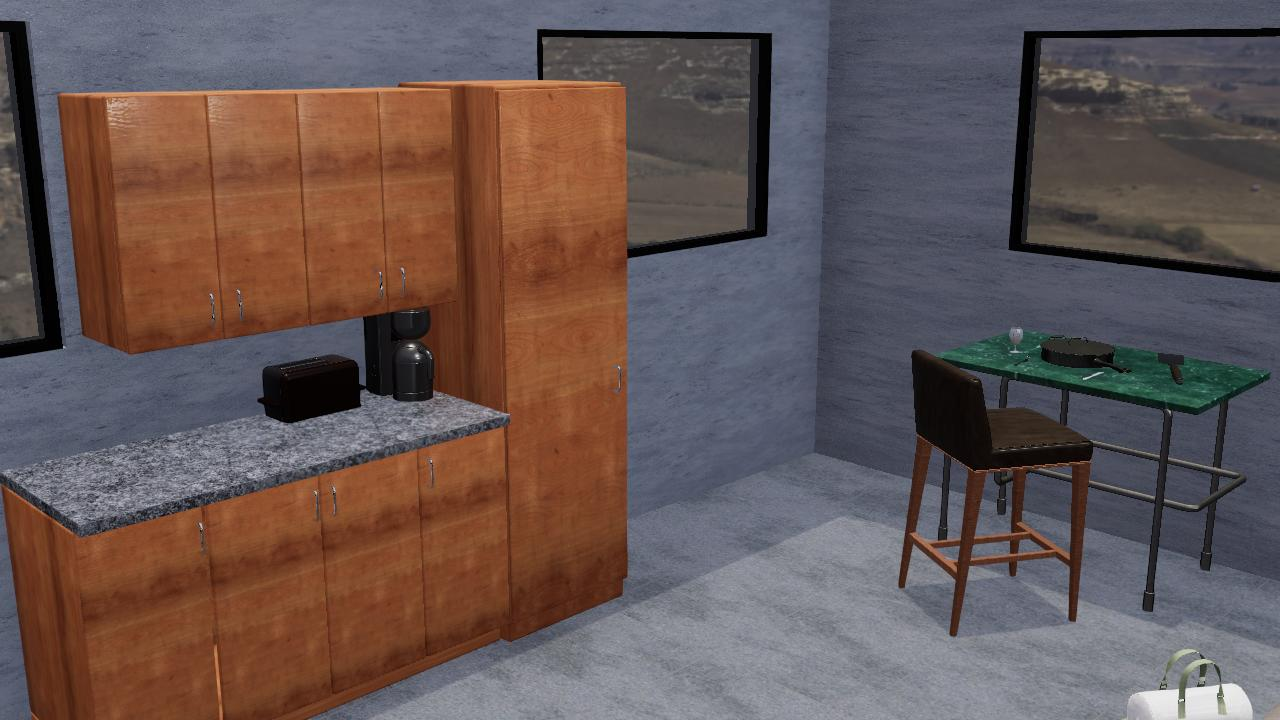
\includegraphics[width=\textwidth]{figures/omnigibson/tdw_sample.jpg}
% \caption{ThreeDWorld: $3.37\pm1.23$}
% \end{subfigure}
% \begin{subfigure}{.19\textwidth}
% 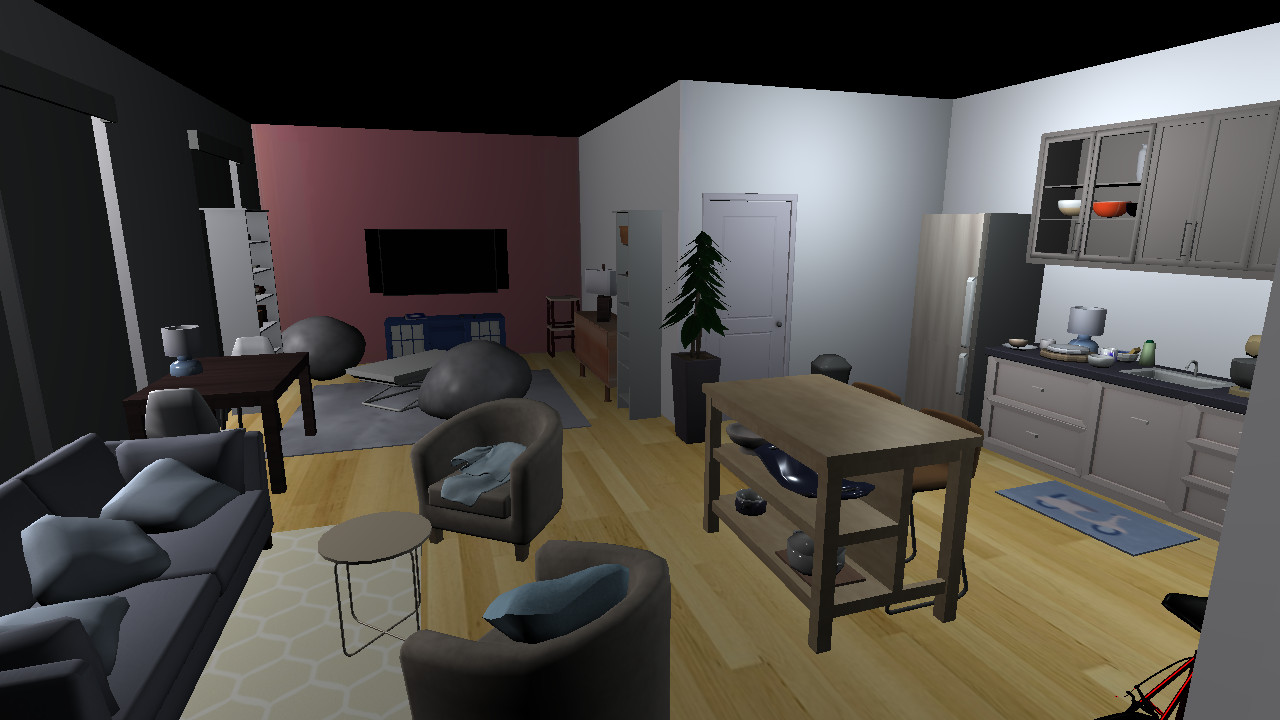
\includegraphics[width=\textwidth]{figures/omnigibson/habitat_sample.png}
% \caption{Habitat2.0: $3.27\pm1.32$}
% \end{subfigure}
% \begin{subfigure}{.19\textwidth}
% 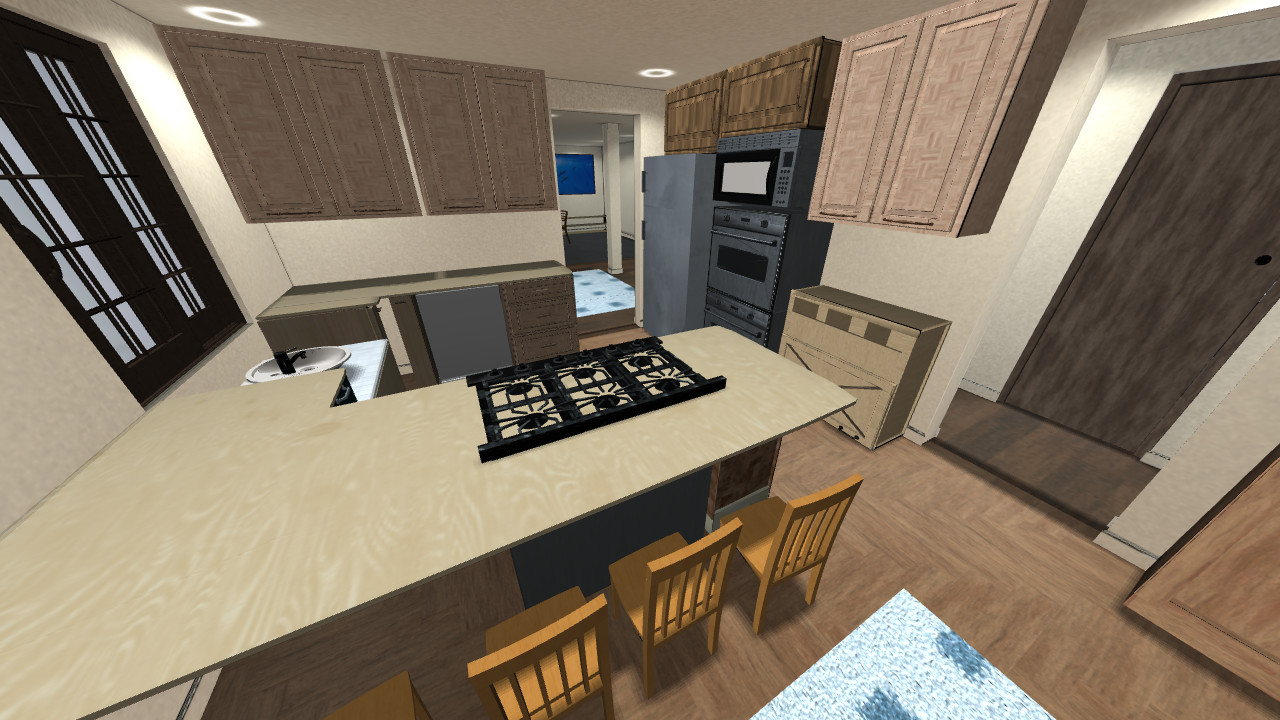
\includegraphics[width=\textwidth]{figures/omnigibson/ig2_sample.png}
% \caption{iGibson2.0: $3.27\pm1.25$}
% \end{subfigure}
\vspace{15pt}
\caption{\textbf{Comparison of Visual Realism:} We evaluate \simulator's visual realism against other simulation environments by running a survey with 60 human subjects. We ask them to rank the realism of sampled images from each environment with a score of 5 (most realistic) to 1 (least realistic). We report the mean and standard deviation and show a sampled image from the study. We observe that the participants consider \simulator to be significantly more visually realistic than all other environments. See Appendix~\ref{amt_study_appx} for more info.}
\label{fig:sim_render}
\end{figure}

% diversity + realism
%An important characteristic of \oldbenchmark is that it's not bounded to any specific simulation environment~\cite{behinh2}, although a fully functional implementation in iGibson 2.0~\cite{li2021ig2} is provided.
%As we use the same general logic language (BDDL) to define activities, we are able to maintain this benefit in \benchmark.
\oldbenchmark is implemented in iGibson 2.0~\cite{li2021ig2}; however, realistic simulation of the diverse activities in \benchmark is beyond the capability of iGibson 2.0. We present a novel simulation environment, \simulator, that provides the necessary functionalities to support and instantiate \benchmark.
\simulator is built on top of Nvidia Omniverse and PhysX 5, providing the simulation of not only rigid bodies, but also deformable objects, fluids, and flexible materials (see Fig.~\ref{fig:sim_obj_prop}), while generating highly realistic ray-traced or path-traced virtual images (see Fig.~\ref{fig:sim_render}).
These features significantly boost the realism of \benchmark compared to other benchmarks.


Similar to \oldbenchmark, \simulator also simulates additional, non-kinematic extended object states (e.g., temperature, soaked level) based on heuristics (e.g., temperature increases when being next to a heat source that is toggled on). \simulator also implements the functionalities to generate infinite valid physical configurations that satisfy the activities' initial conditions as logical predicates (e.g. \texttt{food} is \texttt{frozen}), and to evaluate their goal conditions (e.g. \texttt{food} is \texttt{cooked} and \texttt{onTop} of a \texttt{plate}, the \texttt{cloth} is \texttt{folded}) based on the object's physical states (pose and joint configuration) and extended states. \revision{\simulator natively supports randomization during scene initialization and can sample amongst object models and their poses/states.} The full details of extended object states and logical predicates that \simulator supports can be found in Appendix~\ref{as:object_states}. 

% However, the current simulators' features are insufficient to fully capture many of \benchmark's key properties, such as fluids, deformables, and high-fidelity rendering. 
% To that end, we present \simulator, a state-of-the-art simulator built upon NVIDIA's Omniverse physics and rendering engine and iGibson's~\cite{li2021ig2} infrastructure that enables \benchmark to be fully realized in simulation. \simulator provides 3 key properties crucial to instantiating \benchmark: (1) Accurate simulation of \textbf{complex physical processes} (Fig.~\ref{fig:sim_obj_prop}), (2) \textbf{visual realism} via high-fidelity, super real-time raytraced rendering (Fig.~\ref{fig:sim_render}), and (3) grounded \textbf{perceptual modules} to drive multi-modal embodied AI research (Fig.~\ref{fig:sim_modalities}). \eric{Do we want to highlight (3) this much? This seems to be a basic requirement of any simulator.}

%\subsection{Simulating Complex Physical Processes}

Many everyday tasks are difficult to simulate because they require modeling complex physical processes, such as folding a towel or pouring a glass of water. \simulator unlocks them by supporting realistic simulation of fluids, deformable bodies, and cloths (see Fig.~\ref{fig:model_vis}). Indeed, without these features, over half of \benchmark activities would not be simulatable, highlighting how crucial these features are for capturing everyday activities. \simulator also captures multiple physical processes that are not natively simulatable by Omniverse, such as baking pies or pureeing vegetables. Aside from the extended states mentioned above, we also design a modular \textit{Transition Machine}, which specifies custom transitions between groups of objects when specified conditions are met. For example, a dough placed inside an oven that reaches a certain temperature threshold will turn into a pie. This further expands \simulator's capacity to simulate complex, realistic activities that would otherwise be intractable to fully simulate physically.

% \subsection{High-Fidelity Rendering for Visual Realism}

% Visual realism has been a key limiting factor of current simulation platforms. While rendering capabilities in other simulators have improved significantly during recent years, the sim2real visual domain gap remains quite evident. \simulator substantially improves current state-of-the-art simulation rendering by providing super real-time raytracing, enabling high-fidelity visuals that include realistic visualization of fluids, transparencies, and lights. Moreover, for even greater visual fidelity, \simulator can also leverage path-tracing to render hyper-realistic images. These features considerably reduce the visual domain gap between simulation and reality, and we measure the relative improvement quantitatively by evaluating \simulator's visual quality against current state-of-the-art embodied AI simulators (Fig.~\ref{fig:sim_render}). \eric{And we will get favorable ratings from MTurks?}

% \subsection{Grounding Agent Interactions via Perceptual Modules}

% \eric{In this section, maybe we can claim we provide realistic agent sensing AND actuation, not just sensing alone}
% \fei{suggest changing subsection title to realistic sensing and actuation}

% \fei{This subsection needs to be grounded in numbers or qualitative results, maybe a figure like relmogen paper figure A.5}
% \simulator is agent-centric, and emphasizes grounded interactions between embodied agents and their environment. To that end, \simulator provides diverse perceptual modules to capture realistic sensor modalities from an agent's perspective, including RGB, Depth, Semantic Segmentation, Normal, and Optical Flow images, in addition to non-visual modalities such as proprioception and Lidar scans (Fig.~\ref{fig:sim_modalities}). \simulator also provides varying abstraction levels for agent action spaces, including low-level control, assistive manipulation, and primitive skill execution. Overall, these modules are intended to be useful to the broad embodied AI research community, with the goal of accelerating breakthroughs on \benchmark.


% \eric{In B100 and iG 2.0, we focus a lot on talking about object-centric physical properties (kinematic and non-kinematic) and unary/binary predicate checking/sampling/update mechanism). Do we want to re-iterate these (with the new states added, of course)?} 


% \simulator increases realism in both precision in physics and quality in visuals,

% \begin{enumerate}
%     \item The diversity of these 1K activities require simulating complex physical phenomena (Fig.~\ref{fig:sim_obj_prop}). Built upon Nvidia's Omniverse and iGibson~\cite{li2021ig2}, OmniGibson supports new features, including particles, deformables, transparency, and mixtures of materials (Fig.~\ref{fig:sim_physics}).
%     \item OmniGibson has extremely high rendering quality, with an option to enable super high quality rendering through path tracing technique (Fig.~\ref{fig:sim_render}). 
%     \item OmniGibson's perceptual module will provide utilities for embodied AI research, such as different visual modalities, including RGB images, depth, semantic / instance segmentation, optical flow, scene graph, etc (Fig.~\ref{fig:sim_modalities}).  
%     \item Rendering speed test results and comparison with other benchmarks. Ideally, we can show that OmniGibson achieves high-quality rendering without sacrificing rendering speed, but this is unknown at this point.  
%     \item Although OmniGibson is the only simulator that can support B1K now, in the future, B1K is simulator agnostic and can be implemented in any simulator that is as powerful as OmniGibson. 
% \end{enumerate}


% \begin{figure}[h]
%     \centering
%     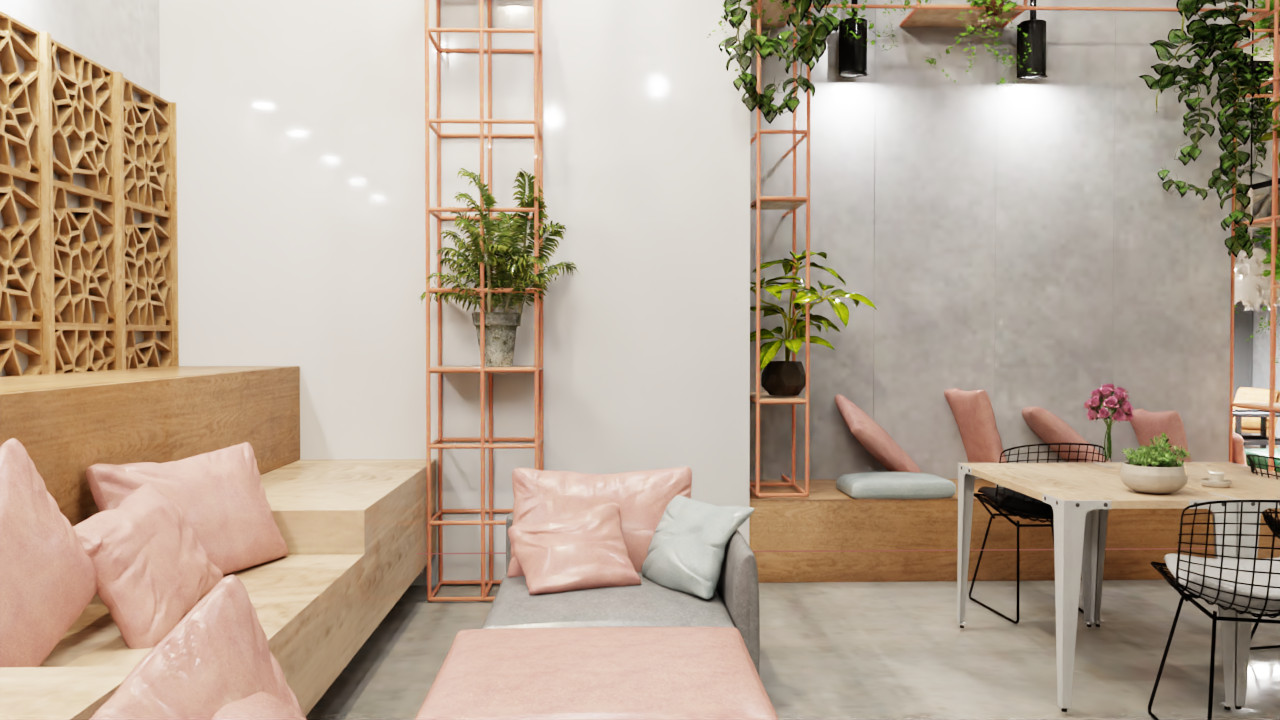
\includegraphics[width=0.19\textwidth]{figures/omnigibson/og_sample.png}
%     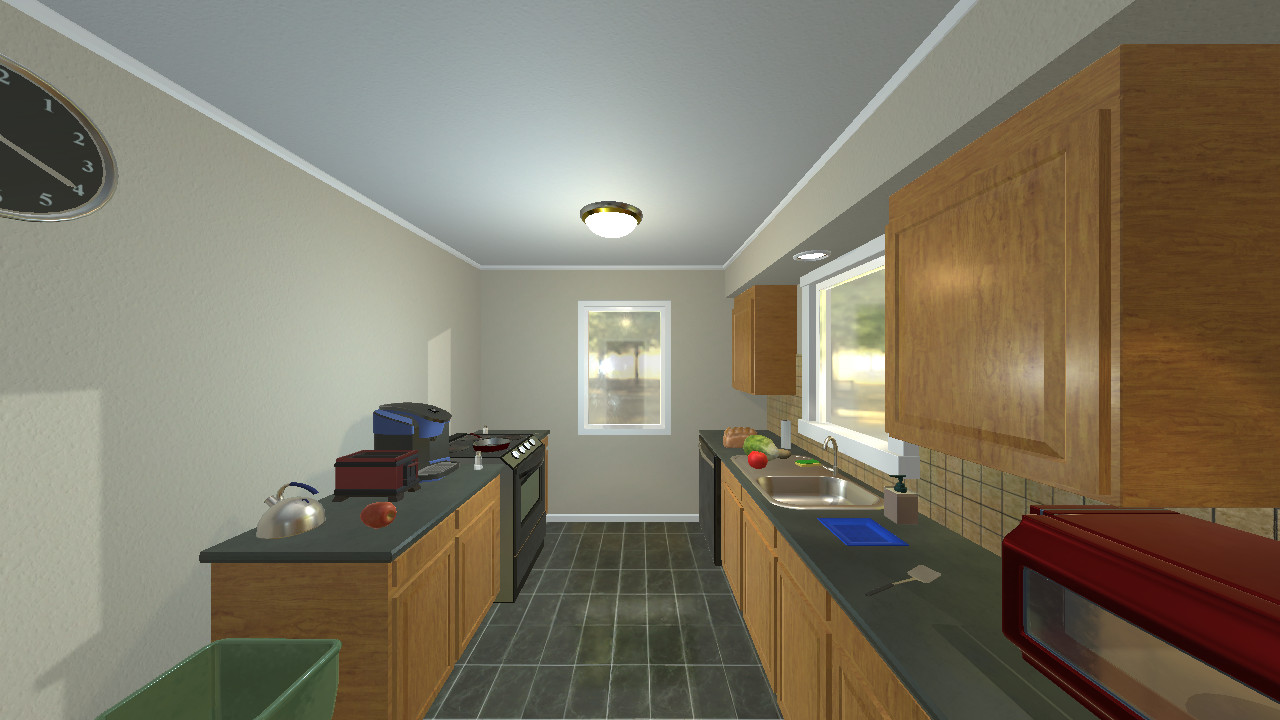
\includegraphics[width=0.19\textwidth]{figures/omnigibson/ai2_sample.png}
%     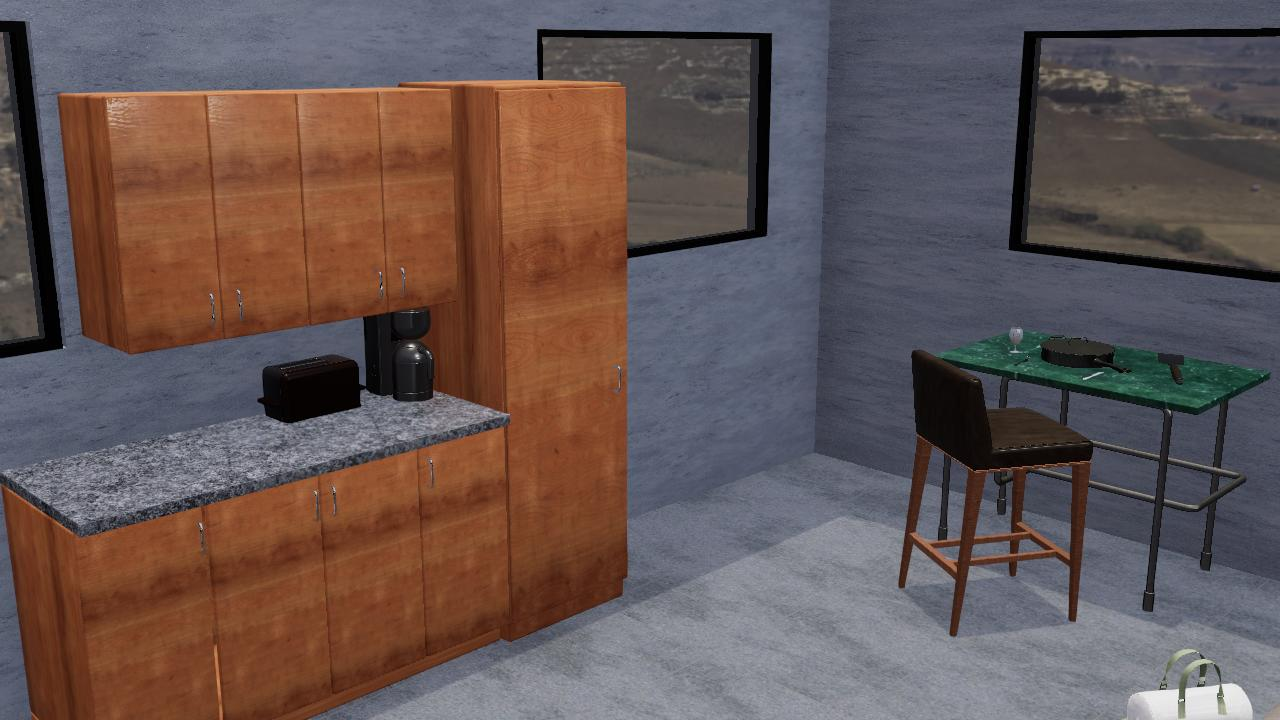
\includegraphics[width=0.19\textwidth]{figures/omnigibson/tdw_sample.jpg}
%     \includegraphics[width=0.19\textwidth]{figures/render_compare_results.png}
%     \includegraphics[width=0.19\textwidth]{figures/render_compare_results.png}
%     \caption{[Comparative][In main body of text] Left: rendering quality example of \simulator, AI2Thor, and ThreeDWorld. Right: we quantify the relative visual realism of \simulator against the other main embodied AI simulators (AI2Thor, ThreeDWorld, Habitat2.0, iGibson2.0) with an AMT study, where subjects were asked to rank randomly sampled images from each simulator in order of realism. We find that \simulator performs XXX \josiah{TODO! Once we have results}.}
%     %\caption{[Comparative][In main body of text] (a) Side-by-side comparison of rendering quality: OmniGibson, OmniGibson-path tracing (super high quality but slow), iGibson, Habitat, AI2. The figures of other benchmarks will come from their demo videos, but OmniGibson will still be visually better than them. (b) Quantitative results for the AMT study showing that OmniGibson is the most realistic judging by humans.}
%     \label{fig:sim_render}
% \end{figure}


% \begin{figure}[h]
% \scalebox{0.96}{
% \captionsetup[subfigure]{labelformat=empty}
% \centering

% \sbox{\bigpicturebox}{%
%   \begin{subfigure}[b]{.49\textwidth}
%   \scalebox{1}[1.2]{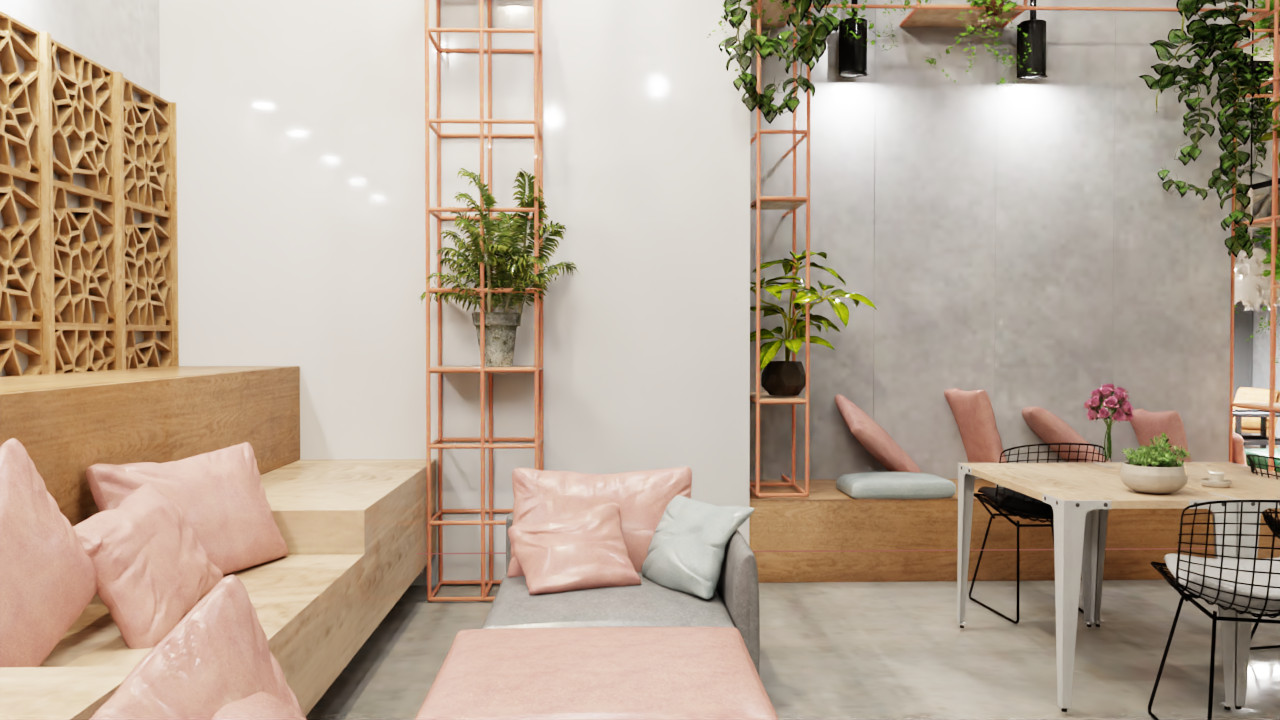
\includegraphics[width=\textwidth]{figures/omnigibson/og_sample.png}}%
% \caption{\textbf{OmniGibson: $\mathbf{1.82\pm1.24}$}}
% \end{subfigure}\hspace{0.3cm}
% }


% \usebox{\bigpicturebox}\hfill
% \begin{minipage}[b][\ht\bigpicturebox][s]{.50\textwidth}
% \begin{subfigure}{.49\textwidth}
% 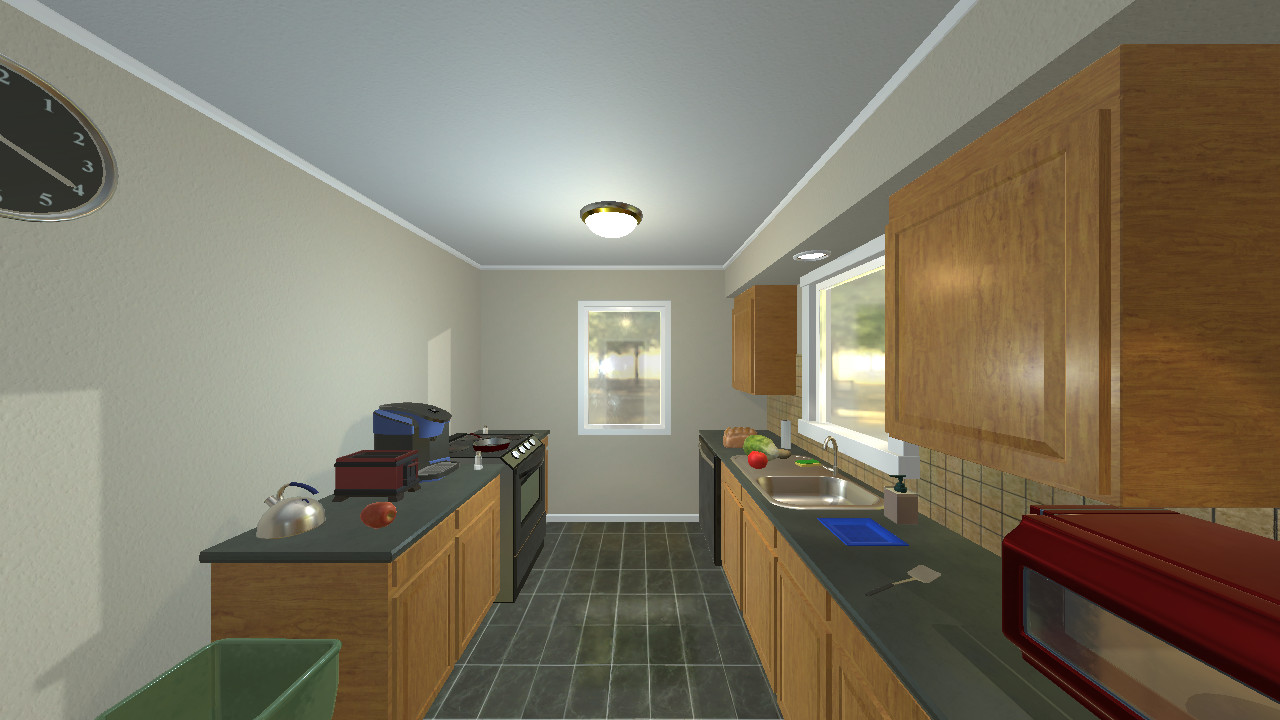
\includegraphics[width=\textwidth]{figures/omnigibson/ai2_sample.png}
% \caption{AI2Thor: $3.27\pm1.25$}
% \end{subfigure}\hfill
% \begin{subfigure}{.49\textwidth}
% 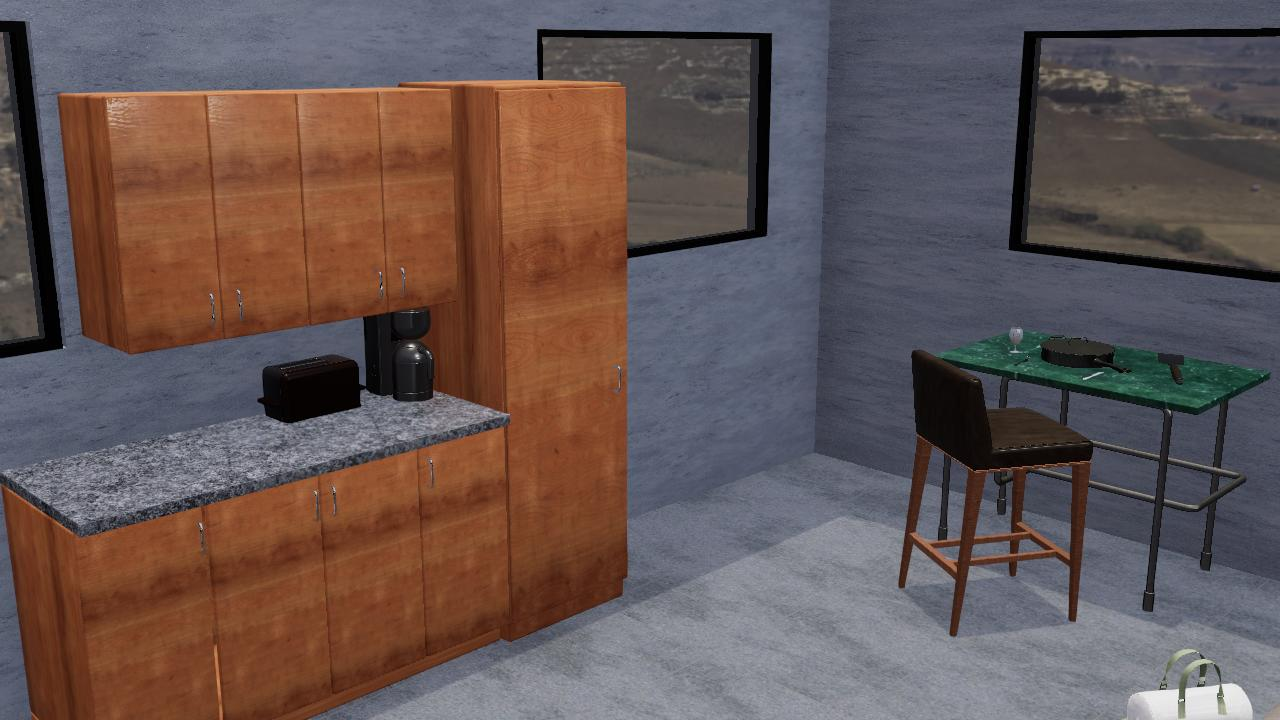
\includegraphics[width=\textwidth]{figures/omnigibson/tdw_sample.jpg}
% \caption{ThreeDWorld: $3.37\pm1.23$}
% \end{subfigure}

% \vfill

% \begin{subfigure}[b]{.49\textwidth}
% 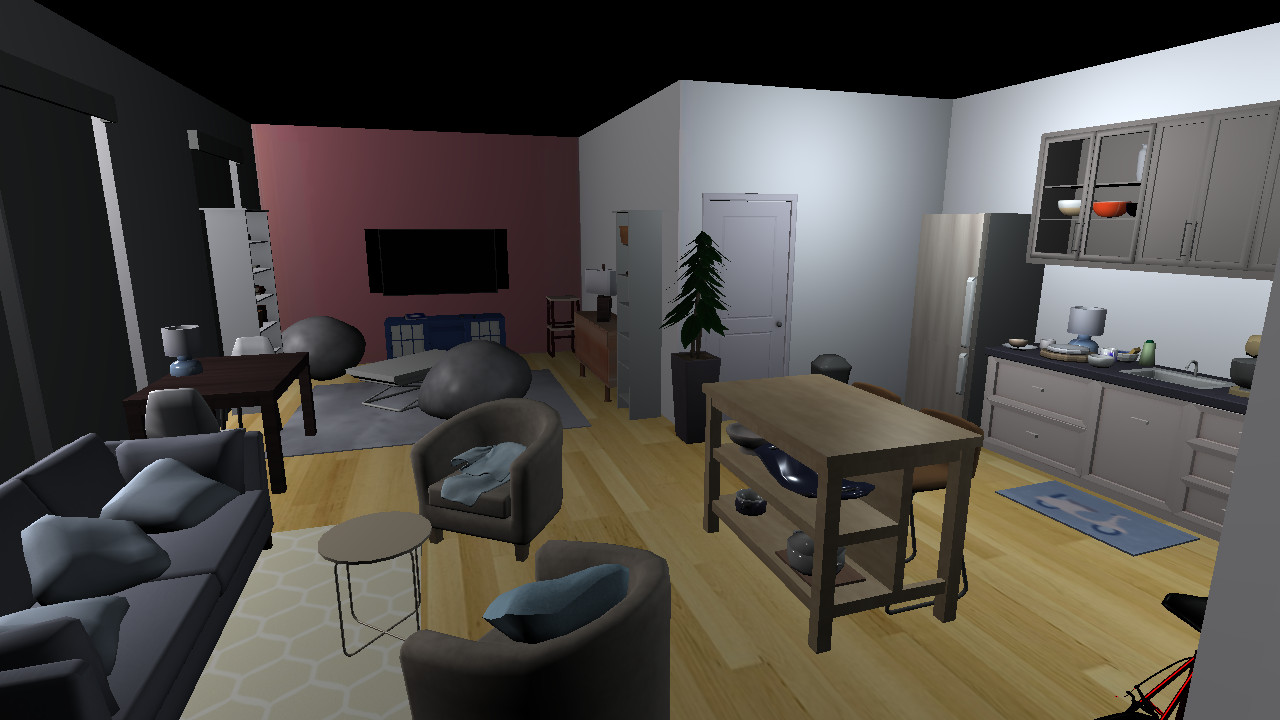
\includegraphics[width=\textwidth]{figures/omnigibson/habitat_sample.png}
% \caption{Habitat2.0: $3.27\pm1.32$}
% \end{subfigure}\hfill
% \begin{subfigure}[b]{.49\textwidth}
% 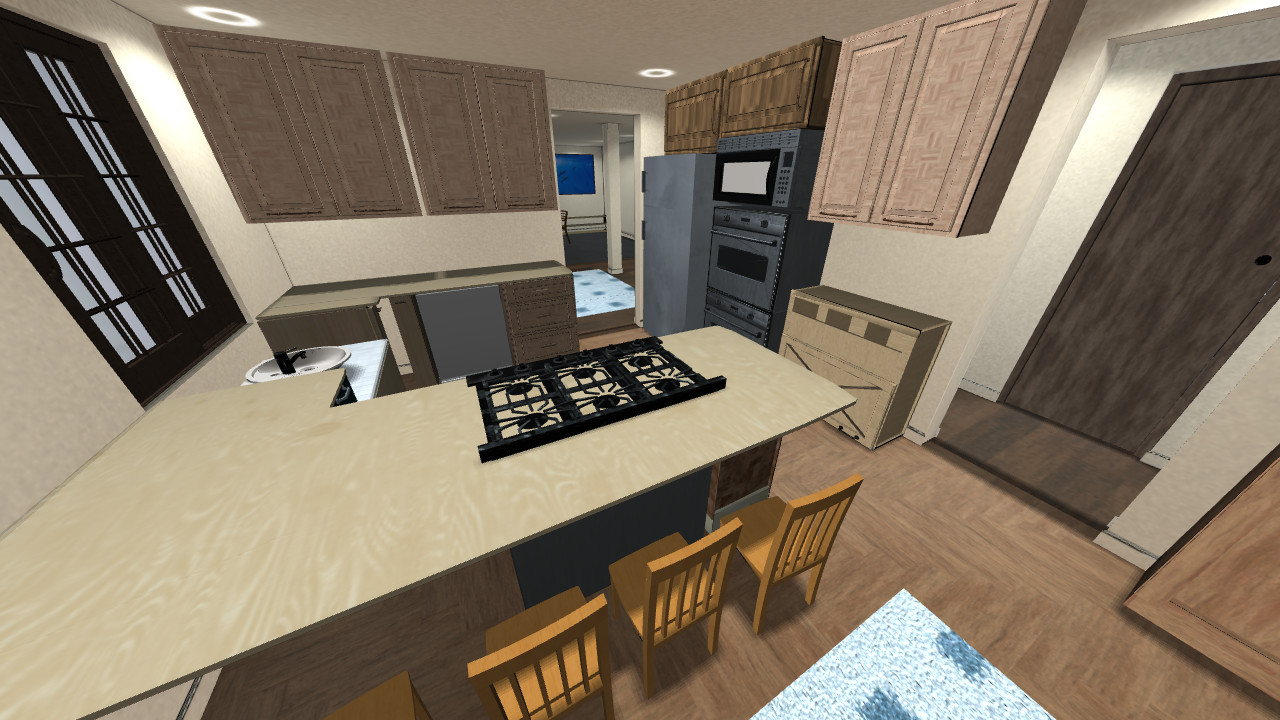
\includegraphics[width=\textwidth]{figures/omnigibson/ig2_sample.png}
% \caption{iGibson2.0: $3.27\pm1.25$}
% \end{subfigure}
% \end{minipage}
% }
% \caption{We evaluate \simulator's visual realism compared to alternative simulation environments by running a survey with 50 human participants to rank the realism of sampled images from each respective environment in order of 1 (most realistic) to 5 (least realistic). We report the resulting mean and standard deviation for each environment, as well as a sampled image from the study, and find that the survey participants consider \simulator to be significantly more realistic compared to all other environments.}

% \label{fig:sim_render}

% \end{figure}


% \sbox{\bigpicturebox}{%
%   \begin{subfigure}[b]{.49\textwidth}
%   \scalebox{1}[1.2]{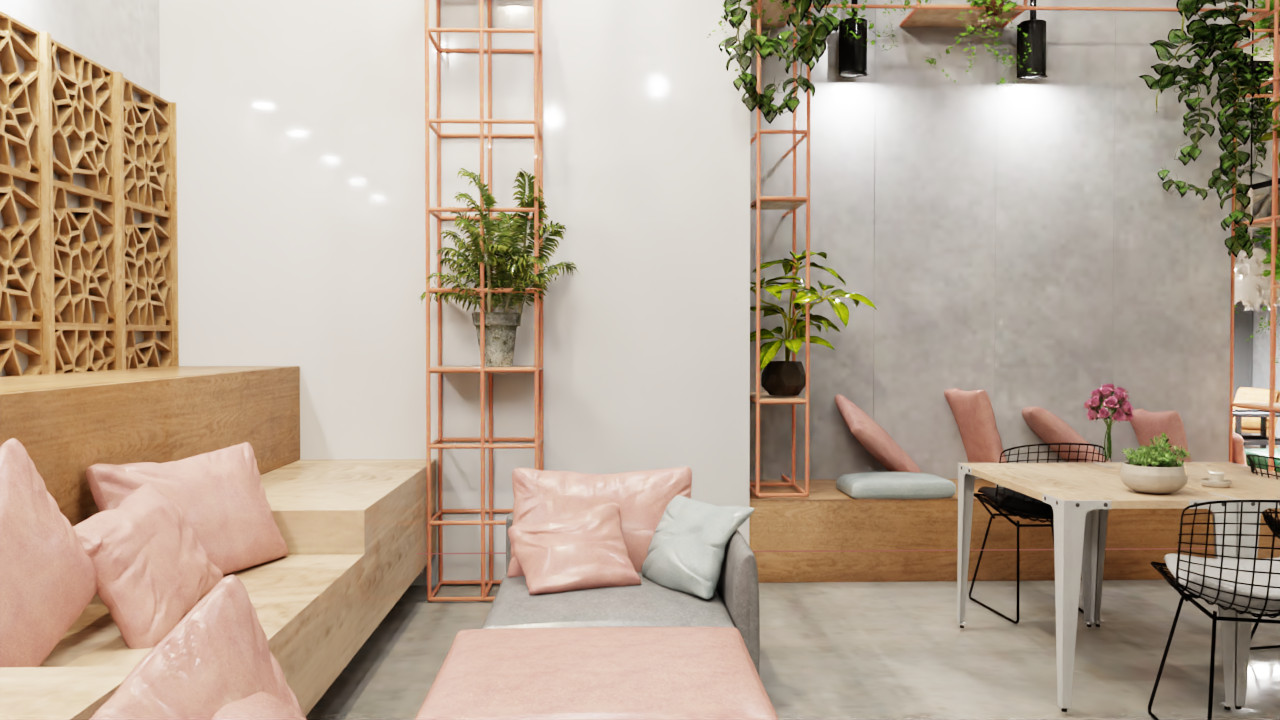
\includegraphics[width=\textwidth]{figures/omnigibson/og_sample.png}}%
% \caption{\textbf{OmniGibson: $\mathbf{1.82\pm1.24}$}}
% \end{subfigure}\hspace{0.3cm}
% }


% \usebox{\bigpicturebox}\hfill
% \begin{minipage}[b][\ht\bigpicturebox][s]{.50\textwidth}
% \begin{subfigure}{.49\textwidth}
% 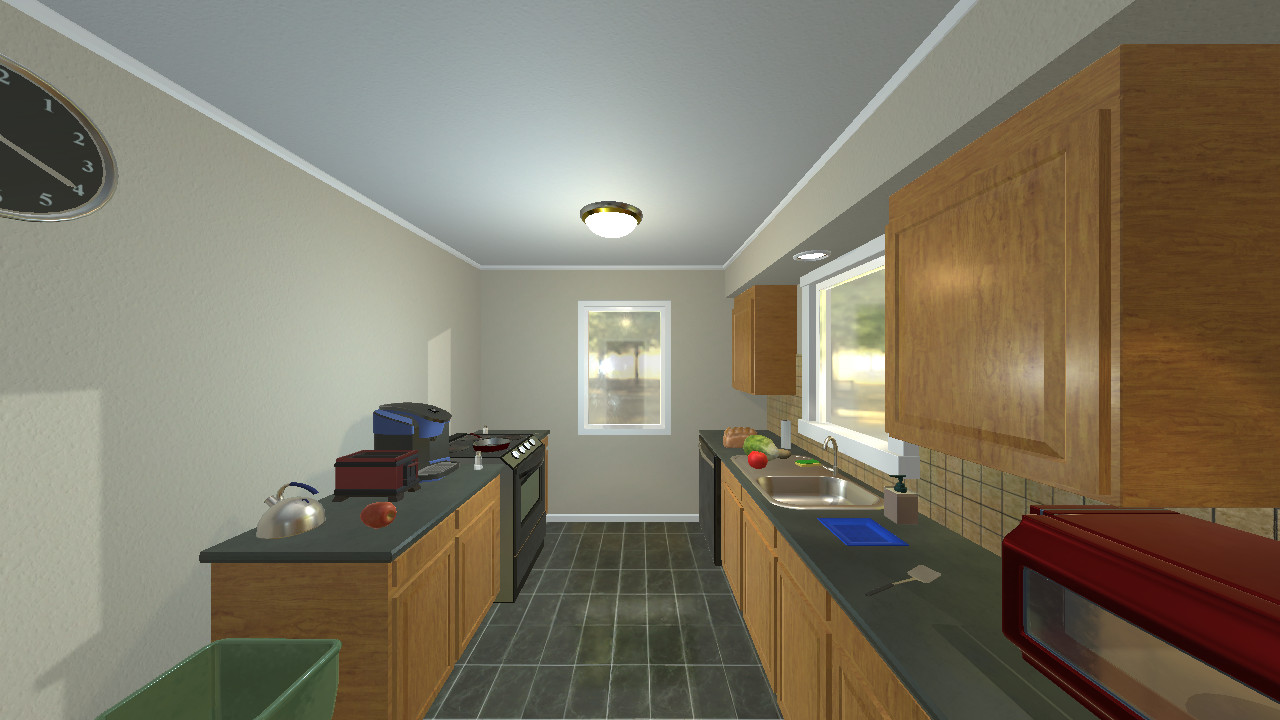
\includegraphics[width=\textwidth]{figures/omnigibson/ai2_sample.png}
% \caption{AI2Thor: $3.27\pm1.25$}
% \end{subfigure}\hfill
% \begin{subfigure}{.49\textwidth}
% 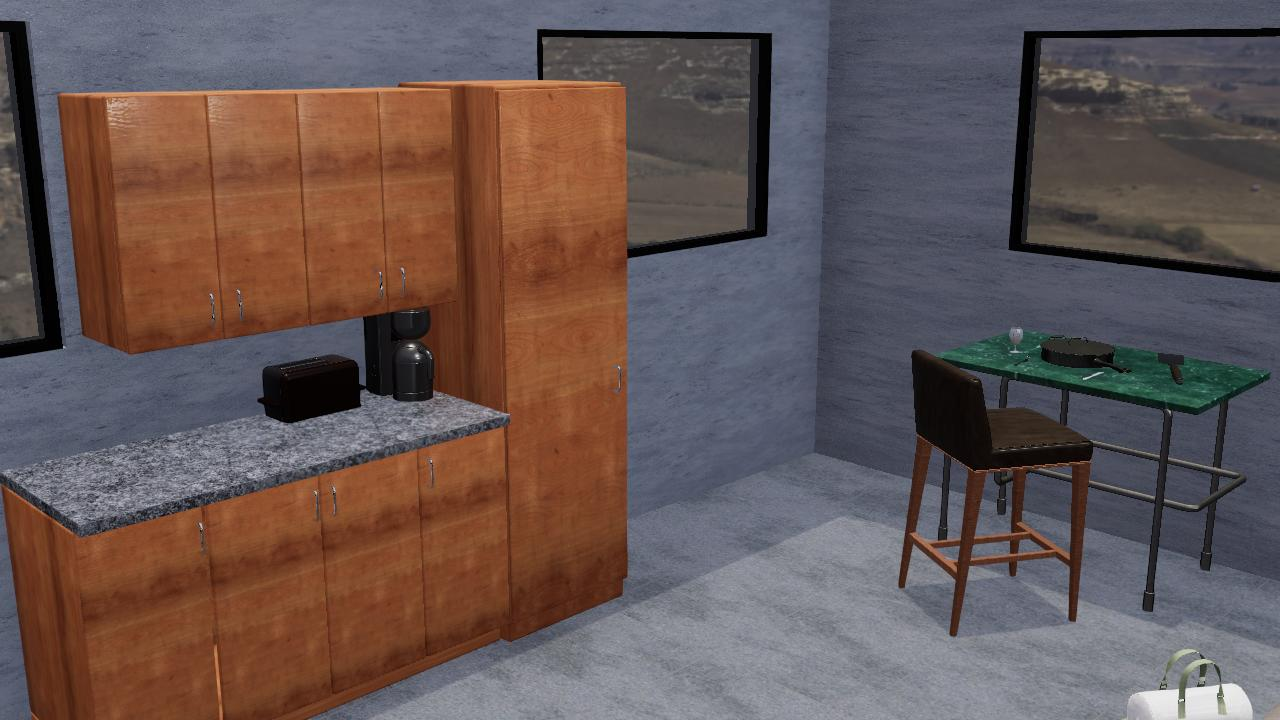
\includegraphics[width=\textwidth]{figures/omnigibson/tdw_sample.jpg}
% \caption{ThreeDWorld: $3.37\pm1.23$}
% \end{subfigure}

% \vfill

% \begin{subfigure}[b]{.49\textwidth}
% 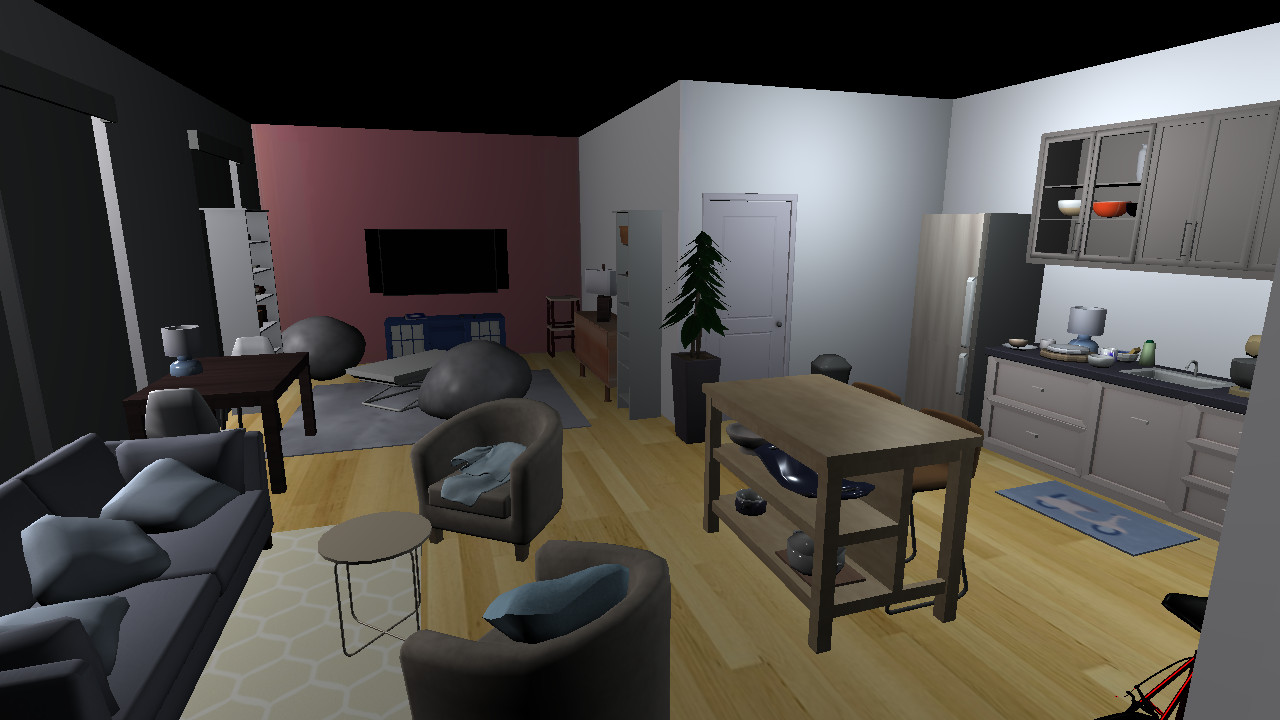
\includegraphics[width=\textwidth]{figures/omnigibson/habitat_sample.png}
% \caption{Habitat2.0: $3.27\pm1.32$}
% \end{subfigure}\hfill
% \begin{subfigure}[b]{.49\textwidth}
% 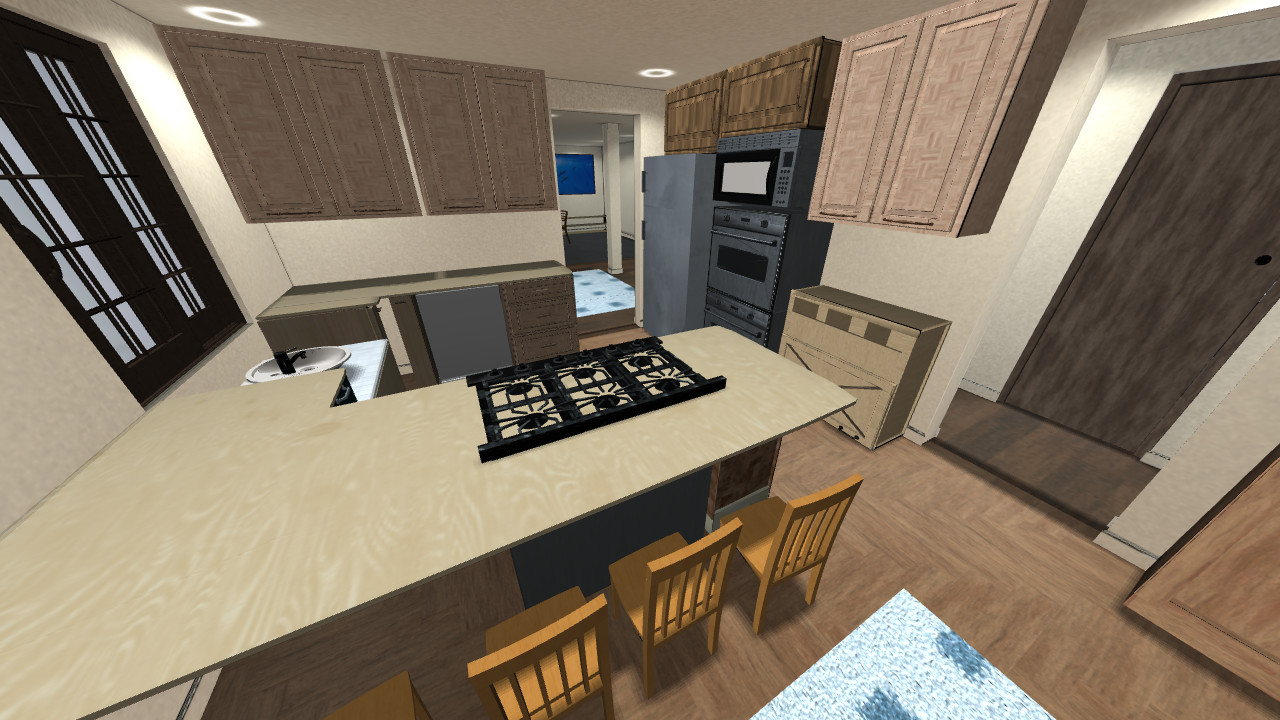
\includegraphics[width=\textwidth]{figures/omnigibson/ig2_sample.png}
% \caption{iGibson2.0: $3.27\pm1.25$}
% \end{subfigure}
% \end{minipage}
% }




% \begin{figure}
% \centering

% \sbox{\bigpicturebox}{%
%   \begin{subfigure}[b]{.45\textwidth}
%   \scalebox{1}[1.2]{\includegraphics[width=\textwidth]{example-image}}%
% \caption{Big picture}
% \end{subfigure}
% }

% \usebox{\bigpicturebox}\hfill
% \begin{minipage}[b][\ht\bigpicturebox][s]{.45\textwidth}
% \begin{subfigure}{.45\textwidth}
% \includegraphics[width=\textwidth]{example-image-a}
% \caption{Small figure}
% \end{subfigure}\hfill
% \begin{subfigure}{.45\textwidth}
% \includegraphics[width=\textwidth]{example-image-b}
% \caption{Small figure}
% \end{subfigure}

% \vfill

% % \begin{subfigure}[b]{.45\textwidth}
% % \includegraphics[width=\textwidth]{example-image-c}
% % \caption{Small figure}
% % \end{subfigure}


% \begin{subfigure}[b]{.45\textwidth}
% \includegraphics[width=\textwidth]{example-image-a}
% \caption{Small figure}
% \end{subfigure}\hfill
% \begin{subfigure}[b]{.45\textwidth}
% \includegraphics[width=\textwidth]{example-image-b}
% \caption{Small figure}
% \end{subfigure}

% \end{minipage}

% \end{figure}



% To conclude, \simulator is a realistic simulator that supports a set of diverse features required to simulate \benchmark activities (see Fig.~\ref{fig:sim_obj_prop}). Although OmniGibson is the only simulator that can support B1K now, in the future, B1K is simulator agnostic and can be implemented in other simulators. 

\begin{figure}[t]
    \centering
    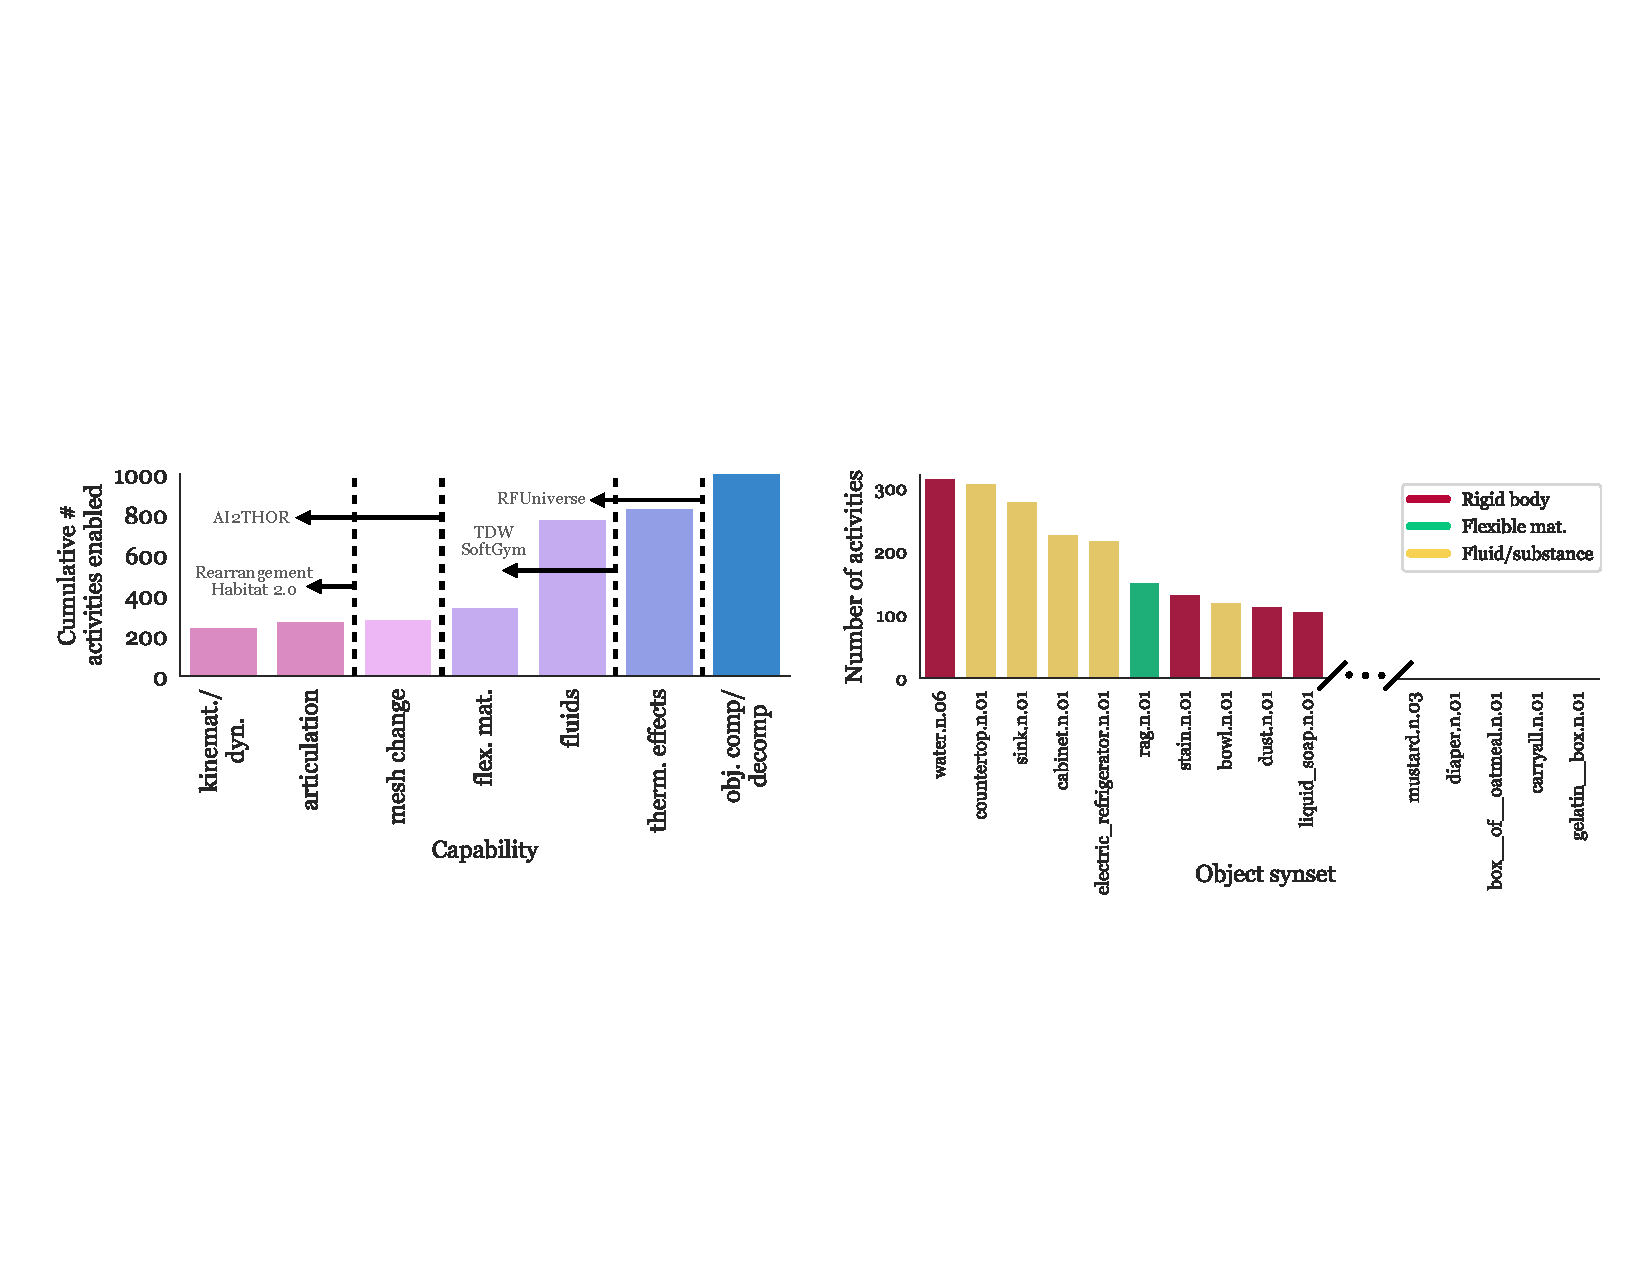
\includegraphics[width=1\textwidth]{figures/object-activity-figs-2024.pdf}\\
    \caption{\textbf{Objects and States in Activity Definitions:} Left: the number of activities unlocked by each simulation capability that \simulator has. None of the other simulation environments are sufficient to fully support \benchmark, e.g. Habitat 2.0 can support only 23\% of the activities. Right: the number of activities that require each object synset (category). Several top-10 object synsets are fluids and flexible materials, necessitating the development of \simulator. As we expect, the object synsets also follow a long-tail distribution: most objects are involved in only a few activities.}
    \vspace{10pt}
    \label{fig:sim_obj_prop}
\end{figure}

